\documentclass{sigchi}

% Use this section to set the ACM copyright statement (e.g. for
% preprints).  Consult the conference website for the camera-ready
% copyright statement.

% Copyright
\CopyrightYear{2020}
%\setcopyright{acmcopyright}
%\setcopyright{acmlicensed}
%\setcopyright{rightsretained}
%\setcopyright{usgov}
%\setcopyright{usgovmixed}
%\setcopyright{cagov}
%\setcopyright{cagovmixed}
% DOI
%\doi{https://doi.org/10.1145/3313831.XXXXXXX}
% ISBN
%\isbn{978-1-4503-6708-0/20/04}
%Conference
%\conferenceinfo{CHI'20,}{April  25--30, 2020, Honolulu, HI, USA}
%Price
%\acmPrice{\$15.00}

% Use this command to override the default ACM copyright statement
% (e.g. for preprints).  Consult the conference website for the
% camera-ready copyright statement.

%% HOW TO OVERRIDE THE DEFAULT COPYRIGHT STRIP --
%% Please note you need to make sure the copy for your specific
%% license is used here!
% \toappear{
% Permission to make digital or hard copies of all or part of this work
% for personal or classroom use is granted without fee provided that
% copies are not made or distributed for profit or commercial advantage
% and that copies bear this notice and the full citation on the first
% page. Copyrights for components of this work owned by others than ACM
% must be honored. Abstracting with credit is permitted. To copy
% otherwise, or republish, to post on servers or to redistribute to
% lists, requires prior specific permission and/or a fee. Request
% permissions from \href{mailto:Permissions@acm.org}{Permissions@acm.org}. \\
% \emph{CHI '16},  May 07--12, 2016, San Jose, CA, USA \\
% ACM xxx-x-xxxx-xxxx-x/xx/xx\ldots \$15.00 \\
% DOI: \url{http://dx.doi.org/xx.xxxx/xxxxxxx.xxxxxxx}
% }

% Arabic page numbers for submission.  Remove this line to eliminate
% page numbers for the camera ready copy
% \pagenumbering{arabic}

% Load basic packages
\usepackage{balance}       % to better equalize the last page
\usepackage{graphics}      % for EPS, load graphicx instead 
\usepackage[T1]{fontenc}   % for umlauts and other diaeresis
\usepackage{txfonts}
\usepackage{mathptmx}
\usepackage[pdflang={en-US},pdftex]{hyperref}
\usepackage{color}
\usepackage{booktabs}
\usepackage{textcomp}

% Some optional stuff you might like/need.
\usepackage{microtype}        % Improved Tracking and Kerning
% \usepackage[all]{hypcap}    % Fixes bug in hyperref caption linking
\usepackage{ccicons}          % Cite your images correctly!
% \usepackage[utf8]{inputenc} % for a UTF8 editor only

% If you want to use todo notes, marginpars etc. during creation of
% your draft document, you have to enable the "chi_draft" option for
% the document class. To do this, change the very first line to:
% "\documentclass[chi_draft]{sigchi}". You can then place todo notes
% by using the "\todo{...}"  command. Make sure to disable the draft
% option again before submitting your final document.
\usepackage{todonotes}

% Paper metadata (use plain text, for PDF inclusion and later
% re-using, if desired).  Use \emtpyauthor when submitting for review
% so you remain anonymous.
\def\plaintitle{Einsatzzwecke von Edge Computing bei autonomen Fahrzeugen}
\def\plainauthor{Florian Mold}
\def\emptyauthor{}
\def\plainkeywords{edge computing; self driving cars; autonomous driving}
\def\plaingeneralterms{Documentation, Standardization}

% llt: Define a global style for URLs, rather that the default one
\makeatletter
\def\url@leostyle{%
  \@ifundefined{selectfont}{
    \def\UrlFont{\sf}
  }{
    \def\UrlFont{\small\bf\ttfamily}
  }}
\makeatother
\urlstyle{leo}

% To make various LaTeX processors do the right thing with page size.
\def\pprw{8.5in}
\def\pprh{11in}
\special{papersize=\pprw,\pprh}
\setlength{\paperwidth}{\pprw}
\setlength{\paperheight}{\pprh}
\setlength{\pdfpagewidth}{\pprw}
\setlength{\pdfpageheight}{\pprh}

% Make sure hyperref comes last of your loaded packages, to give it a
% fighting chance of not being over-written, since its job is to
% redefine many LaTeX commands.
\definecolor{linkColor}{RGB}{6,125,233}
\hypersetup{%
  pdftitle={\plaintitle},
% Use \plainauthor for final version.
%  pdfauthor={\plainauthor},
  pdfauthor={\emptyauthor},
  pdfkeywords={\plainkeywords},
  pdfdisplaydoctitle=true, % For Accessibility
  bookmarksnumbered,
  pdfstartview={FitH},
  colorlinks,
  citecolor=black,
  filecolor=black,
  linkcolor=black,
  urlcolor=linkColor,
  breaklinks=true,
  hypertexnames=false
}

% create a shortcut to typeset table headings
% \newcommand\tabhead[1]{\small\textbf{#1}}

% End of preamble. Here it comes the document.
\begin{document}

\title{\plaintitle}

\numberofauthors{1}
\author{%
  \alignauthor{Florian Mold\\
    %\affaddr{Leitermayergasse 31/12} \\
    %\affaddr{1180 Wien} \\
    \email{e11776836@student.tuwien.ac.at}} \\
}

\maketitle

\begin{abstract}
Das Aufkommen von autonomen Fahrzeugen stellt die IT-Welt vor ganz neue Herausforderungen. Die komplexen IoT-Systeme in den Vehikeln produzieren eine riesige Menge an Daten. Die Rechenkapazität hat sich in den letzten Jahren enorm gesteigert, während die Bandbreite von Netzwerken unverändert geblieben ist. Mit einem zentralen Paradigma wie Cloud Computing, lässt sich das enorme Datenaufkommen nicht mehr bewältigen. Alle Informationen, die ein autonomes Fahrzeug produziert, müssten an ein entferntes Rechenzentrum übertragen, verarbeitet und zurückgesendet werden. Dies führt zu langen Antwortzeiten, was im Falle eines Unfalls katastrophale Folgen haben könnte. Edge Computing ist ein neues Paradigma, welches jene Probleme adressiert. Daten werden direkt bei den Erzeugern verarbeitet und nur das Notwendigste wird an ein Rechenzentrum übertragen. Damit kann die Antwortzeit deutlich verringert werden. Der dezentrale Ansatz eignet sich perfekt für autonomes Fahren. Beispielsweise können die Daten der Verkehrskameras der Autos in Echtzeit verarbeitet und somit schneller auf kritische Situationen reagiert werden. In dieser Arbeit werden Probleme von autonomen Vehikeln, sowie mögliche Einsatzzwecke von Edge Computing beschrieben.
\end{abstract}


\iffalse
% Abieten CM Classfication

\begin{CCSXML}
    <ccs2012>
    <concept>
    <concept_id>10003120.10003121</concept_id>
    <concept_desc>Human-centered computing~Human computer interaction (HCI)</concept_desc>
    <concept_significance>500</concept_significance>
    </concept>
    <concept>
    <concept_id>10003120.10003121.10003125.10011752</concept_id>
    <concept_desc>Human-centered computing~Haptic devices</concept_desc>
    <concept_significance>300</concept_significance>
    </concept>
    <concept>
    <concept_id>10003120.10003121.10003122.10003334</concept_id>
    <concept_desc>Human-centered computing~User studies</concept_desc>
    <concept_significance>100</concept_significance>
    </concept>
    </ccs2012>
    \end{CCSXML}
    
    \ccsdesc[500]{Human-centered computing~Human computer interaction (HCI)}
    \ccsdesc[300]{Human-centered computing~Haptic devices}
    \ccsdesc[100]{Human-centered computing~User studies}
\fi

% Author Keywords
\keywords{\plainkeywords}

\iffalse
    % Print the classficiation codes
    \printccsdesc
    Please use the 2012 Classifiers and see this link to embed them in the text: \url{https://dl.acm.org/ccs/ccs_flat.cfm}
\fi

\section{Einleitung}
Dieses Kapitel beginnt mit der Einführung in das Thema Edge Computing und Autonomes Fahren. Anschließend wird die Motivation dieser Arbeit beschrieben. Daraufhin wird die Zielsetzung und Methodik beschrieben. Am Ende wird noch ein grober Überblick über den Aufbau der Arbeit gegeben.

\subsection{Problemstellung}
Ein autonomes Fahrzeug muss Datenmengen von bis zu 2 Gigabyte die Sekunde in Echtzeit bearbeiten \cite{architectures:2017}. Cloud Computing hat in den vergangenen Jahren die IT-Welt dominiert. Internet of Things (IoT) Geräte produzieren immer mehr Daten und stellen ein Problem für den zentralen Ansatz der Cloud dar. Die potentielle Rechenleistung von Geräten ist stark gestiegen, während die Netzwerkbandbreite gleich geblieben ist. Dadurch wird das Netzwerk zum Flaschenhals für Cloud Computing \cite{promise-edge-computing:2016}. Ebenso wichtig ist der Schutz der übertragenen Daten, welcher sich mit dem Einsatz eines zentralen Paradigmas nicht ordentlich umsetzen lässt  \cite{vision-challenges:2016}. Durch Edge Computing könnten die Herausforderungen von autonomen Fahrzeugen bewältigt werden \cite{opportunities-challenges:2019}.

\subsection{Motivation und Zielsetzung}
Das Ziel der Arbeit ist die Herausarbeitung von potentiellen Möglichkeiten, die der Einsatz von Edge Computing im Vergleich zu Cloud Computing bei autonomen Fahrzeugen ermöglicht. Aktuelle Problematiken, welche den flächendeckenden Einsatz von autonomen Fahrzeugen behindern, werden beleuchtet und wie diese potentiellen Schwachstellen durch die Verwendung von Edge Computing ausgeräumt werden können.

\subsection{Aufbau der Arbeit}
Die Arbeit gliedert sich in dieses Einleitungskapitel, sowie ein theoretisches Kapitel und praktisches Kapitel. Am Ende folgt eine Zusammenfassung und ein Ausblick. In Kapitel \ref{chap:theoretic-part} werden die theoretischen Grundlagen dieser Arbeit behandelt. Dabei wird die Notwendigkeit von Edge Computing, aufgrund der Schwächen von Cloud Computing beschrieben. Daraufhin wird auf autonomes Fahren im Allgemeinen eingegangen und Probleme, die dieser neue Mobilitätsansatz mit sich bringt. In Kapitel \ref{chap:edge-computing-autonomic-cars} werden die Einsatzzwecke von Edge Computing in autonomen Fahrzeugen beschrieben. Kapitel \ref{chap:discussion} und \ref{chap:summary} bilden den Abschluss und fassen die Arbeit nochmals zusammen und geben einen Ausblick über zukünftige Entwicklungen.

\section{Theoretischer Teil} \label{chap:theoretic-part}
In diesem Kapitel werden die theoretischen Aspekte der Arbeit behandelt. Zu Beginn wird das allgemeine Konzept von Cloud Computing erläutert. Dabei werden die Probleme von Cloud Computing herausgearbeitet. Daraus folgend wird die grundsätzliche Idee von Edge Computing beschrieben und wie die Nachteile der Cloud ausgemerzt werden sollen. Zum Abschluss wird autonomes Fahren allgemein beschrieben und welche Problematiken dabei entstehen.

\subsection{Cloud Computing}
Cloud Computing hat die IT-Landschaft in der vergangenen Dekade dominiert und bringt zwei nennenswerte Vorteile mit sich. Erstens bietet die Zentralisierung, Größenvorteile zur Senkung von Kosten und die Anzahl der Administrator/innen. Zweitens müssen Organisationen kein Rechenzentrum bauen und anschließend warten, dadurch, dass diese Rechenleistung und Speicher mieten \cite{emergence-edge-computing:2017}. Entwickler/innen mussten keine physische Infrastruktur mehr verwalten, jedoch hat sich der Aufwand der Wartung von virtueller Infrastruktur vervielfacht \cite{cloud-programming-simplified:2019}. Diese Faktoren haben dazu geführt, dass Rechenkapazität in riesigen Rechenzentren, über den Globus verteilt, aggregiert wurde \cite{emergence-edge-computing:2017}. Alle Berechnungen in die Cloud zu verschieben war ein sehr effizienter Ansatz, da im Rechenzentrum deutlich mehr Rechenkapaztiät zur Verfügung steht, als bei Geräten am Rand des Netzwerks. Während die Datenverarbeitungsgeschwindigkeit stark gestiegen ist, hat sich die Geschwindigkeit der Netzwerkinfrastruktur nicht wirklich gesteigert. Daraus folgend, dass Geräte immer mehr Daten erzeugen, wird das Netzwerk zum Flaschenhals von Cloud Computing werden. In einem selbstfahrenden Auto müssen visuelle Informationen in Echtzeit verarbeitet werden. Wenn ein Fahrzeug nun Daten für die weitere Verarbeitung an ein Rechenzentrum sendet, wäre die Antwortzeit für eine Reaktion in einem Ernstfall, zu lange. Daten am Rand des Netzwerks zu bearbeiten würde zu niedrigeren Antwortzeiten, effizienterer Verarbeitung und zu weniger Auslastung des Netzwerks führen \cite{promise-edge-computing:2016}. Fast alle elektrischen Geräte werden in Zukunft ein Teil des Internet of Things (IoT) werden Daten produzieren sowie konsumieren. Die Zahl der Edge Devices wird sich in einigen Jahre auf mehr als eine Milliarde belaufen. Die unglaubliche Menge an Rohdaten, ist durch Cloud Computing nicht verarbeitbar. Die meisten Daten werden nicht mehr an die Cloud übertragen, sondern direkt am Rand des Netzwerks verarbeitet. Abbildung \ref{fig:cloud-computing} zeigt die herkömmliche Struktur von Cloud Computing. Daten werden erzeugt und ungefiltert an die Cloud übergeben. Benutzer/innen senden eine Anfrage, um die gewünschten Daten zu erhalten. Dieses Paradigma ist nicht ausreichend für IoT, da unnötig viel Bandbreite und Rechenkapazität eingesetzt wird. Zweitens ist der Schutz der Privatsphäre ein Problem des Cloud Computing Ansatzes. IoT-Geräte haben nur beschränkte Energiekapazitäten zur Verfügung und drahtlose Übertragung ist oftmals sehr aufwändig, daher ist die Verlagerung von Berechnungen energiesparsamer \cite{vision-challenges:2016}. Edge Computing ist ein neues Paradigma, welches so eine Dezentralisierung erlaubt \cite{emergence-edge-computing:2017}. 

\begin{figure}
\centering
  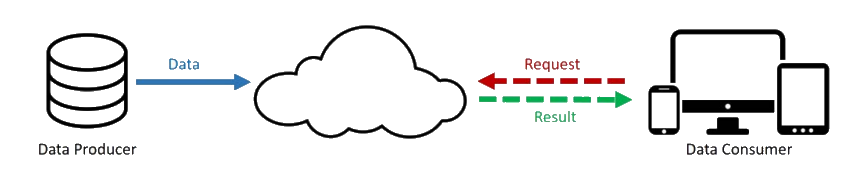
\includegraphics[width=0.75\columnwidth]{figures/cloud-computing-structure.PNG}
  \caption{Cloud Computing Paradigma \cite{vision-challenges:2016}}~\label{fig:cloud-computing}
\end{figure}

\subsection{Edge Computing}
Edge Computing bezeichnet Technologien, die Berechnungen am Rand des Netzwerks durchführen, wie in Abbildung \ref{fig:edge-computing} zu erkennen ist. Speicher- und Rechenressourcen sind in der Nähe von den Erzeugern der Daten, wie beispielsweise Sensoren oder Smartphones. Solche Geräte werden oft als Fog- oder Edge-Nodes bezeichnet. Am Netzwerkrand laden die Geräten nicht nur Daten, sondern verarbeiten, speichern und cachen diese. Um diese Aufgaben bewältigen zu können, muss ein Edge-Gerät folgende Anforderungen wie Differenzierung, Erweiterbarkeit, Isolation und Verlässlichkeit unterstützen \cite{promise-edge-computing:2016}.

\begin{figure}
\centering
  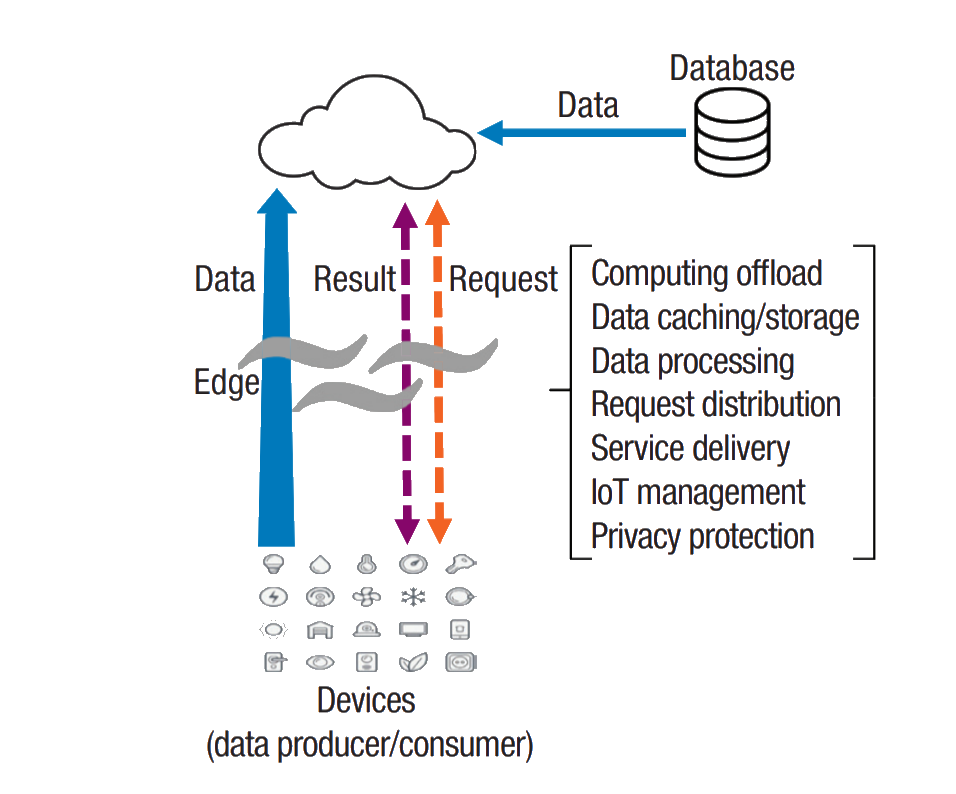
\includegraphics[width=0.75\columnwidth]{figures/edge-computing-structure.PNG}
  \caption{Edge-Geräte fungieren als Konsumenten und Produzenten. Anfragen zwischen der Cloud und den Geräten sind bidirektional. Viele Berechnungen werden direkt am Endgerät ausgeführt \cite{promise-edge-computing:2016}.}~\label{fig:edge-computing}
\end{figure}

Dieser dezentrale Ansatz von Edge Computing könnte viele Vorteile bringen. Folgend werden die vielversprechendsten Gewinne von Edge Computing näher beschrieben: \cite{promise-edge-computing:2016, emergence-edge-computing:2017}

\begin{itemize}
    \item \textbf{Latenz}
     \begin{itemize}
         \item Die physische Nähe der verarbeiteten Geräte zu den erzeugenden Geräten des/der Benutzer/in verringert die Latenz. Durch den dezentralen Ansatz von Edge Computing, verringert sich die benötigte Netzwerkbandbreite um die Daten an ein Rechenzentrum zu übermitteln. Die Paketverzögerungsvariation oder der Netzwerk-Jitter werden ebenso deutlich reduziert. Zudem sinkt, aufgrund des verringerten Aufwands, der Energieverbrauch. Die so eben genannten Verbesserungen durch Edge Computing sind wertvoll für Anwendungsfälle, die eine geringe Latenz voraussetzen, wie Argumented Reality (AR) oder selbstfahrende Autos
     \end{itemize}
    \item \textbf{Skalierbarkeit}
         \begin{itemize}
            \item Ein Großteil der gesammelten Datenmengen muss nicht an die Cloud übertragen werden. Edge-Geräte bearbeiten die Anfragen direkt lokal und senden nur die notwendigsten Daten an ein Rechenzentrum. Die eingehende Netzwerklast von Rechenzentren kann somit um ein Vielfaches reduziert werden.
     \end{itemize}
    \item \textbf{Privatsphäre}
         \begin{itemize}
            \item Dadurch, dass die Verarbeitung der Daten näher bei der Quelle erfolgt, können sensible Daten vor fremden Zugriffen besser geschützt werden. Beispielsweise können für den/die Hersteller/in wichtige Nutzungs- sowie Verhaltensdaten im Vorhinein anonymisiert werden.
     \end{itemize}
    \item \textbf{Robustheit}
         \begin{itemize}
            \item Falls das Cloud-Rechenzentrum durch einen Systemfehler oder einen Angriff ausfallen sollte, dann können Edge-Geräte so einen Ausfall verbergen, indem sie auf Fehlerbehandlungsroutinen zurückgreifen.
        \end{itemize}
\end{itemize}

\subsubsection{Probleme}
Edge Computing braucht sogenannte Killerapplikationen um sein komplettes Potential zu entfalten. Diverse Applikationsarten kommen potentiell in Frage. Dazu zählt der Katastrophenschutz, Körperkameras für Polizeibeamte, intelligente Fahrzeuge und Gesundheitssysteme \cite{promise-edge-computing:2016}.

\begin{itemize}
    \item \textbf{Programmierbarkeit}
    \begin{itemize}
        \item Funktionen von Edge Computing Anwendungen müssen zwischen der Cloud und dem Netzwerkrand aufgeteilt werden. Aktuelle Ansätze sind manuell balanciert worden. Dieser Ansatz ist jedoch nicht skalier- order erweiterbar. Daraus folgend entsteht eine Notwendigkeit für einfache Programmierframeworks und Tools.
    \end{itemize}
    \item \textbf{Namensgebung}
        \begin{itemize}
            \item Aktuell gibt es noch kein effizientes Schema um Geräte am Netzwerkrand so zu benennen, damit sie einfach gefunden werden können. Edge Computing braucht ein eindeutiges Benennungsschema, das mit mobilen Geräten, dynamischer Topologie und dem Schutz der Privatspähre umgehen kann, während das Netzwerk skalierbar bleibt.
        \end{itemize}
    \item \textbf{Privatsphäre und Sicherheit}
        \begin{itemize}
            \item Auch wenn durch Edge Computing einige Sicherheitsprobleme von Cloud Computing eliminiert werden können, existieren trotzdem potentielle Sicherheitsprobleme. Ein Hacker könnte durch die Analyse von diversen Smart-Home Daten feststellen, ob das Haus leersteht und damit Einbrüche planen.
        \end{itemize}
\end{itemize}

\subsection{Autonomes Fahren}
In den vergangenen Jahren wurden viele Ressourcen in die Entwicklung von selbstfahrenden Fahrzeugen investiert. Im Mittelpunkt des autonomen Fahrens steht die Schaffung einer künstlichen Intelligenz. Bereits 2020 sollen bemannte und fahrerlose Fahrzeuge koexistieren. Aufgrund der durchschnittlichen Lebensspanne von Autos soll diese Phase etwa 20 Jahre dauern. Neue Verkehrssysteme für autonome Fahrzeuge werden nach und nach installiert werden. 2040 und darüber hinaus sollen alle Fahrzeuge komplett Fahrerlos sein. Pro Jahr sterben mehrere Millionen Menschen im Straßenverkehr. Autonome Fahrzeuge, sollen diese Zahl auf fast null reduzieren \cite{drive-my-car:2017}. Viele Automobilhersteller und Unternehmen in der Transportbranche, wie Uber, Ford, Delphi, Volkswagen, Audi, General Motors, BMW und noch einige weitere, haben bereits angekündigt bis zum Jahre 2030, ihre eigenen selbstfahrenden Autos auszuliefern \cite{driverless-future:2016}.

\subsubsection{Probleme}
So vielversprechend die Technologie bereits ist, können einige Probleme die flächendeckende Einführung von selbstfahrenden Autos verzögern. Folgende Probleme können identifiziert werden:

\begin{itemize}
    \item Softwarequalitätsbedenken
        \begin{itemize}
            \item Wie jedes technisches Gerät, dass mit dem Internet verbunden ist, könnten auch selbstfahrende Autos Opfer von Hackingangriffen werden. 2015 haben zwei Personen eine Sicherheitslücke in einem Chrysler ausgenutzt und damit die Kontrolle über das Fahrzeug erlangt. Die Beiden konnten auf die Klimaanlage, das Radio, den Scheibenwischer, die Lenkung und den Motor zugreifen, sowie die Bremsen betätigen. Dabei handelte es sich zwar nicht um ein autonomes Fahrzeug, aber ähnliche und erweiterte Features werden auch in der neuen Generation der Mobilität zu finden sein. Problematisch könnte sein, wenn autonome Fahrzeuge kein Eingreifen durch den Fahrer mehr zulassen \cite{privacy-and-security-issues:2019}.
    \end{itemize}
    \item Rechtliche Probleme
        \begin{itemize}
            \item Damit selbstfahrende Autos auf den Straßen unterwegs sein dürfen, sind zusätzliche rechtliche Rahmenbedingungen nötig. Fahrerlizenzen könnten in Zukunft angepasst oder überflüssig werden. Des Weiteren ist die Schuldfrage bei autonomen Fahrzeugen nicht einfach zu klären. Wer übernimmt Verantwortung im Falle eines Unfalls. Bei bemannten Fahrzeugen ist diese Frage schnell geklärt, bei autonomen Fahrzeugen sind jedoch mehr Parteien involviert. Beispielsweise könnten die Hersteller der Hard- bzw. Software zur Verantwortung gezogen werden. Eine weitere Möglichkeit wäre die Verantwortlichmachung der Hersteller der Straßentechnologie \cite{itf:2015}.
        \end{itemize}
    \item Privatsphäre und Datenverwendung
        \begin{itemize}
            \item Ein Faktor, den diese neue Technologie mit sich bringt, ist der Verwendungszweck von den gesammelten Daten. Zuerst sollte bereits im Vorhinein für alle Hersteller/innen festgelegt werden, welche Daten gesammelt werden dürfen. Aus den Daten, die ein selbstfahrendes Auto sammelt, kann geschlossen, werden wo jemand wie lange mit wem war. Es sollte festgelegt werden, wer Zugriff auf diese Daten haben darf. Beispielsweise könnten die Daten für die Polizei oder den Staat interessant sein \cite{glancy-privacy:2012}.
        \end{itemize}
\end{itemize}

\section{Edge Computing in autonomen Fahrzeugen} \label{chap:edge-computing-autonomic-cars}
Das Hauptziel des Einsatzes von Edge Computing in autonomen Fahren ist Sicherheit. Diese Aufgaben ist schwer bewältigbar, da ein autonomes Auto eine Menge an Daten in Echtzeit bearbeiten muss (bis zu 2GB/s) \cite{architectures:2017}. Ein selbstfahrendes Auto muss einige Sekunden vor dem Eintritt eine potentielle Gefahr erkennen und reagieren. Je schneller die komplexen Berechnungen vom Edge System durchgeführt würden, desto sicherer ist das Fahrzeug. Autonome Fahrzeuge benötigen eine Menge komplexer Technologie \cite{opportunities-challenges:2019}.
Ein vollständig autonomes Auto muss die Umwelt Wahrnehmen und mithilfe von vielen Sensoren navigieren. Zu diesen Sensoren zählt das Globale Positionsbestimmungssystem (GPS) und die Laser Imaging Detection (LiDAR), eine inertiale Messeinheit (IMU) sowie diverse Kameras. Um so viele Sensordaten zu verarbeiten ist eine komplexe Rechnerstruktur vonnöten. Aktuelle Prototypen haben mehrere hochwertige Graphic Processing Units (GPUs) und Central Processing Units (CPUs) \cite{architectures:2017}. Für die Kommunikation zwischen Modulen mit geringem Overhead braucht man ein leichtgewichtiges Betriebssystem. Des Weiteren müssen eine enorme Menge an Daten in Echtzeit bearbeitet werden. Diese Daten kommen von unterschiedliche Sensoren und sind heterogen. Da es sich oftmals um mobile Systeme handelt, haben die Geräte eine beschränkte Energieaufnahme \cite{opportunities-challenges:2019}. 

In Abbildung \ref{fig:edge-computing-drive-infrastructure} ist der Aufbau von selbstfahrenden Autos in Kombination mit Edge Computing dargestellt. Jedes Fahrzeug ist mit einem Edge Computing System ausgestattet, welches alle Module wie Lokalisierung, Wahrnehmung, Planung und Kontrolle beinhaltet. Jedes dieser Fahrzeuge kann mit Edge Servern und mit der Cloud durch existierende Mobilkommunikationsnetzwerke kommunizieren \cite{opportunities-challenges:2019}.

\begin{figure}
\centering
  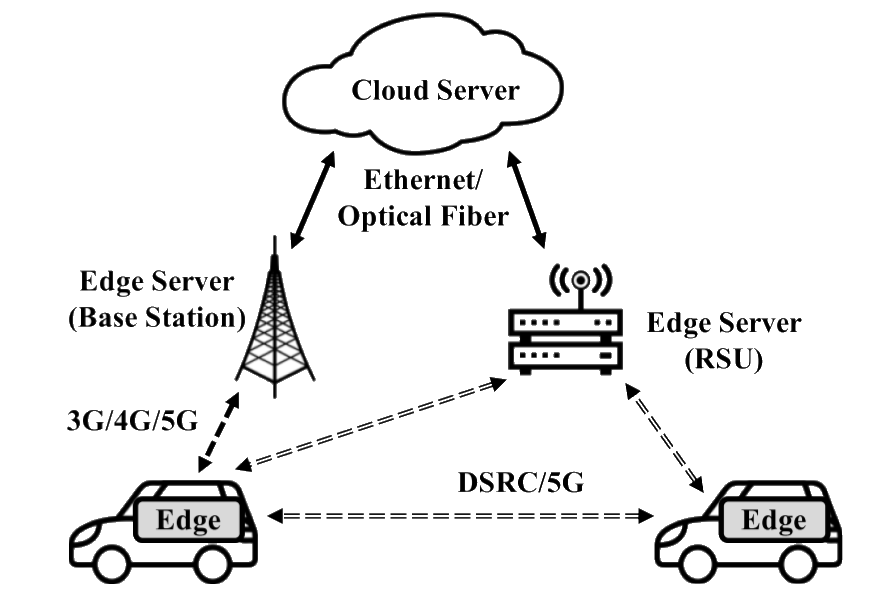
\includegraphics[width=0.75\columnwidth]{figures/edge-computing-drive-infrastructure.PNG}
  \caption{Autonomes Fahren mit Edge Computing Unterstützung \cite{opportunities-challenges:2019}.}~\label{fig:edge-computing-drive-infrastructure}
\end{figure}

\subsection{Einsatzzwecke}
Edge Computing hat eine Menge unterschiedlicher Einsatzzwecke in der Automobilindustrie. Folgend werden einige Möglichkeiten genannt.

\subsubsection{Sensordaten}
Ein modernes Fahrzeug besitzt hunderte Sensoren. Obwohl viele Daten bereits im Auto verarbeitet werden, muss dennoch einiges an die Cloud übertragen werden. Mit Edge Computing kann die Anzahl der Daten limitiert werden. Die meisten Daten können direkt verarbeitet werden und nicht sensitive Daten müssen nicht an die Cloud übertragen werden. Dadurch werden die Datenübertragungskosten reduziert und sensitive Daten verlassen das Auto nicht \cite{role-edge-computing:2020}.

\subsubsection{Elektrofahrzeuge}
Die Batterie von Elektroautos benötigt konstante Leistung, dazu ist eine fortlaufende Überwachung und eine vorausschauende Wartung der Batterie notwendig. Der Zustand einer Batterie hängt von mehreren Faktoren ab, wie dem Fahrerverhalten, die Verkehrsbedingungen, die Ladezyklen und so weiter. Edge Computing könnte alle diese Daten in Echtzeit sammeln und den/die Besitzer/in, im Falle einer Abweichung, alarmieren \cite{role-edge-computing:2020}. 
%Edge Computing hilft dabei den Ladeprozess zu optimieren .

\subsubsection{Intelligentes Verkehrsmanagement}
In einer futuristischen Kreuzung, können alle Fahrzeuge untereinander kommunizieren, während sie sich der Kreuzung nähern. Ein Edge Gerät kann die Daten der anderen Fahrzeuge abfragen und weiß somit bereits im Vorhinein über die Situation bescheid. Daraus resultierend kann der Verkehrsdurchsatz einer Kreuzung gesteigert werden \cite{role-edge-computing:2020}.

\subsubsection{Infotainment}
Edge Computing kann die Benutzerfahrung deutlich verbessern, indem es die Anwendungen und Schnittstellen, welche der/die Benutzer/in verwendet, versteht. Dann kann festgestellt werden, wo das Benutzerinterface Verbesserungspotential bietet \cite{role-edge-computing:2020}. 

%Machine Learning Modelle können durchgehend Daten sammeln, verarbeiten und analysieren. Diese Machine Learning Algorithmen können direkt auf einem Edge Gerät betrieben werden, um das Verhalten des Benutzers zu analysieren. 

\subsubsection{Authentifizierung}
Multi-Level Authentifizierung kann durch Kameras und Sensoren ermöglicht werden. Die Kameras im Fahrzeug könnten für Gesichtserkennung genutzt werden. Bluetooth Geräte für die Erkennung des Smartphones des/der Besitzer/in. Dadurch könnte die unerlaubte Nutzung von Fahrzeugen oder der Diebstahl von Fahrzeugen reduziert \cite{role-edge-computing:2020}.

\subsubsection{Fahrzeugflottenmanagement}
Ein/e Flottenmanager/in muss alle Fahrzeugdaten seiner Flotte im Auge behalten. Wenn ein Fahrzeug auf eine Reise geschickt wird, dann soll es nicht bereits nach kurzer Zeit gewartet werden müssen. Edge Computing kann solche Situationen vorhersehen, indem Sensordaten mit Machine Learning Modellen analysiert werden. Die Geräte können angeben, wie viele Kilometer noch gefahren werden können \cite{role-edge-computing:2020}.

\subsubsection{Wartung}
Edge Computing kann einige Parameter des Fahrzeuges überwachen. Dazu zählt die Umgebungstemperatur, die Kilometeranzahl, die Reifenabnutzung, die Bremsabnutzung, die Beschleunigung und die Geschwindigkeit. Es kann vorhergesagt werden, wann eine Komponente ausfallen könnte und den/die Besitzer/in informieren. Wenn beispielsweise der Reifendruck zu niedrig ist, dann wird der/die Fahrer/in alarmiert \cite{role-edge-computing:2020}.

\subsubsection{Vehikel zu Vehikel Kommunikation}
Jedes autonome Fahrzeug wird Daten über die Straßenbeschaffenheit, Wetterveränderungen mit anderen Fahrzeugen teilen. Dadurch ermöglicht man anderen Fahrzeugen rechtzeitig über potentielle Gefahren wie Umleitungen, Trümmer, Unfälle und Überschwemmungen informiert zu werden und entsprechende Gegenmaßnahmen zu ergreifen. Ein Großteil dieser Daten wird zwischen den Fahrzeugen selbst gesendet und empfangen werden können, ohne dass sie mit entfernten Rechenzentren kommunizieren müssen. Diese Kommunikation macht jedes Fahrzeug auf der Straße zu einer Erweiterung der Sensoren jedes anderen Fahrzeugs und liefert somit die bestmöglichen Informationen über die Situation \cite{5-use-cases:2019}.

\subsubsection{Reduzierte Latenz}
Durch die Unterbringung von Servern und Rechenressourcen in Edge-Einrichtungen, die sich sowohl in Gebieten mit hohem Verkehrsaufkommen als auch in weiter entfernten Gebieten mit begrenztem Bandbreitenzugang befinden, kann sichergestellt werden, dass autonome Fahrzeuge mit minimaler Latenzzeit auf die Daten zugreifen können, die sie benötigen, um schnell Entscheidungen treffen zu können. Als IoT-Geräte haben selbstfahrende Vehikel auch die Möglichkeit, ihre eigenen Entscheidungen zu treffen, ohne sich auf die Anleitung von Servern in entfernten Rechenzentren verlassen zu müssen \cite{5-use-cases:2019}.

\subsubsection{Smart City Integration}
Damit autonome Fahrzeuge ihr volles Potenzial entfalten können, müssen städtische Gebiete mit hohem Verkehrsaufkommen in IoT investieren. Sensoren, die Informationen über Straßenzustände bis hin zu Echtzeitberichten über Staus weiterleiten werden gesammelt. "Intelligente Städte" werden autonome Fahrzeuge mit wertvollen Informationen zu versorgen, damit sie bessere und effizientere Entscheidungen treffen können. Durch die Schaffung einer solchen Umgebung mit leichtem Zugang zu lokalen Ressourcen könnten Städte dazu beitragen, das volle Potenzial von IoT-Geräten auszuschöpfen \cite{5-use-cases:2019}.

\section{Diskussion} \label{chap:discussion}
Im Rahmen dieser wissenschaftlichen Arbeit wurden die potentiellen Einsatzzwecke von Edge Computing in selbstfahrenden Autos herausgearbeitet. Dabei konnten einige gewinnbringende Einsatzgebiete von Edge Computing identifiziert werden. Mit den Möglichkeiten der aktuellen IT-Technologien, sind komplett fahrerlose Autos noch nicht denkbar. Jedoch könnten die neuen Möglichkeiten von Edge Computing unbemannte Fahrzeuge in den nächsten 20 Jahren zur Realität werden lassen. Das volle Potential von Edge Computing ist jedoch noch nicht ausgeschöpft. Zukünftig wird Cloud Computing durch Edge Computing als das dominierende Paradigma abgelöst werden.

\section{Zusammenfassung und Ausblick} \label{chap:summary}
Dieses Kapitel fasst die wichtigsten Ideen und Ergebnisse dieser Arbeit zusammen und gibt einen Ausblick über zukünftige Entwicklungen.

\subsection{Zusammenfassung}
Autonome Fahrzeuge produzieren mit ihren unzähligen Sensoren eine enorme Menge an Daten. Das dezentrale Paradigma Edge Computing ist sehr vielseitig und bietet eine Menge von Einsatzmöglichkeiten in autonomen Fahrzeugen. Dazu zählt beispielsweise die Überwachung des internen Zustands des Fahrzeugs oder die Kommunikation mit anderen Vehikeln, um über die Verkehrslage informiert zu werden.

\subsection{Ausblick}
Edge Computing birgt großes Potential für die Zukunft. Die Datenmengen, welche von der rasant wachsenden Anzahl von IoT-Geräten produziert werden, stellen im aktuellen Kontext eine große Herausforderung dar. Für die Verarbeitung dieser Datenflut existiert noch keine ordentliche Lösung. Wenn mehr Forschungsaufwand in Edge Computing investiert wird, dann könnte dieser Ansatz eine potentielle Antwort sein. Vielseitige Einsatzzwecke von Edge Computing sind Smart Cities, der Finanzsektor, das Gesundheitswesen oder Argumented Reality sind denkbar \cite{5-use-cases-1:2019}.


% BALANCE COdge ComputingLUMNS
\balance{}

% REFERENCES FORMAT
% References must be the same font size as other body text.
\bibliographystyle{SIGCHI-Reference-Format}
\bibliography{sample}

\end{document}

%%% Local Variables:
%%% mode: latex
%%% TeX-master: t
%%% End:
